\chapter{Path and navigation}\label{CH:PathNavigation}
This chapter contain the system description of the landing plan generator and the navigation system.
\section{Landing plan}\label{Ch:LandingPlan}
The landing plan consists of two main parts; the landing path and the approach path. The landing path is a straight line path orientated with respect to a reference position, which in this system is the position of the net. The approach path is designed as a lateral Dubins path and a longitudinal straight line path, and ensures that the \gls{uav} is able to enter the landing path at the correct height with the correct orientation.
\subsection{Landing Path}\label{SS:netApproach}
The landing path is inspired by the work done in \citep{Skulstad&Syversen} where waypoints were used to create a straight line path towards the net. The proposed landing path proved successful and the same landing path design is used in this thesis. The decent angle of the straight line path should be kept small to avoid build up in speed. The trade off is that the start height of the landing path must be above any obstacles that is around the landing area. A waypoint is here defined as:
\begin{equation}
\textbf{WPn} = \begin{bmatrix}
x \\
y \\
z
\end{bmatrix}
\end{equation}
where $x,y,z \in \Bbb R^3$. The straight line path is constructed relative to the net as shown in figure \ref{Fig:LandingPhase}, with way-points given as:
\begin{subequations}
\begin{align}
&\mathbf{WP4} = 
\begin{bmatrix}
-a0 \\
0 \\
h_{nc} + a1\tan(\gamma_n) 
\end{bmatrix}\\
&\mathbf{WP3} = 
\begin{bmatrix}
a1 \\
0 \\
h_{nc} - a1\tan(\gamma_n)
\end{bmatrix}\\
&\mathbf{WP2} = \mathbf{WP3} + 
\begin{bmatrix}
a2 \\
0 \\
-a2\tan(\gamma_l)
\end{bmatrix}\\
&\mathbf{WP1} = \mathbf{WP2} + 
\begin{bmatrix}
a3 \\
0 \\
0 \\
\end{bmatrix}
\end{align}
\end{subequations}
where the description of the parameters used is given in table \ref{Tb:Approach Parameters}. The net is placed between the fourth and third way points, where the fourth waypoint is used as a aiming position for the \gls{uav} and avoid transitional behaviour from switching waypoint before hitting the net.
\begin{table}[H]
\begin{center}
    \begin{tabular}{ | l | l |}
    \hline
    \textbf{Parameter} & \textbf{Description} \\ \hline
    $h_{nc}$ & The height from ground to the net center \\ \hline
    $a0$ & The distance behind the net \\ \hline
    $a1$ & The distance in front of the net \\ \hline
    $a2$ & The length of the glide slope \\ \hline
    $a3$ & The length of the approach towards the glide slope \\ \hline
    $\gamma_n$ & The net attack angle \\ \hline
    $\gamma_l$ & The landing glide slope angle \\ \hline
    \end{tabular}
\end{center}
\caption{Landing path parameters }
\label{Tb:Approach Parameters}
\end{table}
Continuing the waypoints are rotated into the NED frame by a rotation around the z-axes.
\begin{equation}
\mathbf{WP}^n = \mathbf{R}(\psi_{net})\mathbf{WP}^b
\end{equation}
were $\psi_{net}$ is the heading of the net, and $\mathbf{R}(\psi_{net})$ is the standard rotation matrix around the z-axis.
\begin{figure}
\def\svgwidth{\textwidth} % Defining the width since Inkscape hasn't done this yet in the .pdf_tex file
\input{InkFig/LandingPhase.pdf_tex}
\caption{The landing path}
\label{Fig:LandingPhase}
\end{figure}

\subsection{Approach path}\label{SS:LandingApproach}
The approach path is separated into two parts; a lateral and longitudinal path. The purpose of the approach path is to ensure that the \gls{uav} can enter the landing path at the correct height with the correct orientation from any initial position. The lateral and longitudinal paths are created separately 
\subsubsection{Lateral path}
The lateral path is designed as a Dubins path. Start pose, $P_s$, is the pose where the landing plan generation request was made. Finish pose, $P_f$ is the start position of the landing path with the orientation towards the net. Dubins path was chosen due to its circular turns, simplistic design and meets the requirement that the \gls{uav} enters the landing path with the correct orientation.

The lateral path is constructed with the equations presented in section \ref{S:DubinsPath}. The standard approach path is the shortest path of the four different rotation pairs given in table \ref{Tb:DubinsTurningDirection}, however when implemented there exits the option of manually setting the rotation direction for both circles. The shortest path is determined by calculating the length of each variants, where the shortest path variant is chosen. The resulting path is shown in figure \ref{Fig:LateralPath}.
\begin{figure}[H]
	\centering
		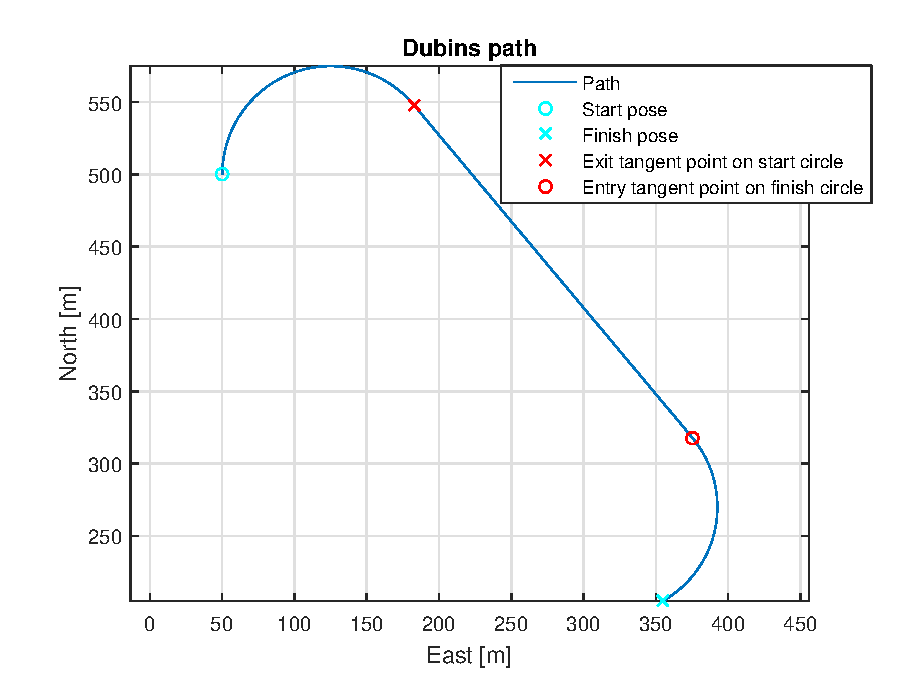
\includegraphics[width=1\textwidth]{figs/SysPlot/DubinsPath.eps}
		\caption{Lateral Dubins path}
		\label{Fig:LateralPath}
\end{figure}

The construction of the lateral path consists of two arc with a straight line between the arcs. The arcs are constructed by first finding the entry and exit angle with respect to the inertia frame, defined as $\psi_0$ and $\psi_1$ respectfully:
\begin{subequations}
\begin{align}
\psi_0 &= \begin{cases}
\atan2(Y_s-Y_{cs},X_s-X_{cs}) & \text{if start circle} \\
\atan2(Y_{P_N}-Y_{cf},X_{P_N}-X_{cf}) & \text{otherwise}
\end{cases}\\
\psi_1 &= \begin{cases}
\atan2(Y_{P_\chi}-Y_{cs},X_{P_{\chi}}-X_{cs}) & \text{if start circle} \\
\atan2(Y_{f}-Y_{cf},X_{f}-X_{cf}) & \text{otherwise}
\end{cases}
\end{align}
\end{subequations}
Further the turn angle must be defined, which is the difference between $\psi_1$ and $\psi_0$. The periodic behaviour of the unit circle must be respected, in addition to the rotation direction. The maximum turning angle is given as:
\begin{equation}
\psi_{max} = \begin{cases}
-|\psi_1 - \psi_0| & \text{if counter clockwise rotation and } \psi_1 - \psi_0 \leq 0 \\
-(2\pi - |\psi_1-\psi_0|) & \text{ if counter clockwise rotation and } \psi_1 - \psi_0 > 0 \\
|\psi_1 - \psi_0| & \text{if clockwise rotation and } \psi_1 - \psi_0 \geq 0 \\
(2\pi - |\psi_1-\psi_0|) & \text{ if clockwise rotation and } \psi_1 - \psi_0 < 0
\end{cases}
\end{equation}
where $|\psi_1-\psi_0| \in(-\pi,\pi]$. From the maximum turning angle the angle step and number of angle segments in the arc can be determined:
\begin{subequations}
\begin{align}
h &= \text{sign}\frac{d_{arc}}{R} \\
N &= \ceil[\Bigg]{\frac{\text{sign}(\psi_{max})\psi_{max}}{|h|}} + 1
\end{align}
\end{subequations}
where $h$ is arc angle step and $N$ the total number of steps in the arc. The step angle must have the same sign as $\psi_{max}$ to ensure the correct rotation direction. Continuing the heading function $\psi(\varpi)$ can be defined as:
\begin{equation}
\psi(\varpi) = \begin{cases}
\psi_{max} & \varpi = N-1 \\
\varpi h & \text{otherwise}
\end{cases}
\end{equation}
where $\varpi = 1,...,N-1$. Finally the arc path can be defined as:
\begin{equation}
\mathbf{p}(\varpi) = \begin{bmatrix}
\mathbf{O}_c \\
\end{bmatrix} + R\begin{bmatrix}
\cos(\psi_0 + \psi(\varpi)) \\
\sin(\psi_0 + \psi(\varpi)) \\
\end{bmatrix}
\end{equation}
A summary of the lateral path is:
\begin{equation}
\mathbf{p}(i) = \begin{cases}
\begin{bmatrix}
\mathbf{O}_{cs} \\
\end{bmatrix} + R_s\begin{bmatrix}
\cos(\psi_{0} + \psi(\varpi)) \\
\sin(\psi_{0} + \psi(\varpi)) \\
\end{bmatrix} & \text{Start circle} \\
\begin{bmatrix}
\mathbf{O}_{cf} \\
\end{bmatrix} + R_f\begin{bmatrix}
\cos(\psi_{0} + \psi(\varpi)) \\
\sin(\psi_{0} + \psi(\varpi)) \\
\end{bmatrix} & \text{Finish circle}
\end{cases}
\end{equation}
where $i \in [1,...,N_s + N_f]$ with $N_s$ and $N_f$ as the number of segments in the start and finish circle respectfully.
\subsubsection{Longitudinal path}
The longitudinal path is designed as a straight line path along the lateral path, which fused together with the lateral path forms a spiral path towards the landing path. The approach path hold a constant decent angle until the correct height is reached, which is defined as the start height for the landing path. The approach decent angle is then adjusted in order for the correct height to be reach. The approach decent angle is defined as:
\begin{equation}
\gamma_d = \begin{cases}
\atan2(\Delta z,||\mathbf{p}(i+1)-\mathbf{p}(i)||_2) & \text{if } \atan2(\Delta z,||\mathbf{p}(i+1)-\mathbf{p}(i)||_2)\leq \gamma_{d_{Max}} \\
\gamma_{d_{Max}}										& \text{otherwise}
\end{cases}
\end{equation}
where $\gamma_{d_{Max}}$ is the maximum decent angle for the approach path, and $\Delta z$ is defined as:
\begin{equation}
\Delta z = z_d-z(i)
\end{equation}
where $z_d$ is the $z$ component in $WP1$. Finally the longitudinal path is included into the approach path, which is given as:
\begin{equation}
\mathbf{r}(i) = \begin{bmatrix}
\mathbf{p}(i) \\
||\mathbf{p}(i)-\mathbf{p}(i-1)||_2\tan(\gamma_d)
\end{bmatrix}
\end{equation}
where $\mathbf{r}(i)$ is the landing path, with $i \in [2,...,N_s+N_f]$ and 
$p = \begin{bmatrix}
x(i) & y(i)
\end{bmatrix}^T$ is the lateral path. The resulting height profile of the approach path is shown in figure \ref{Fig:HeightProfile}.
\begin{figure}[H]
	\centering
		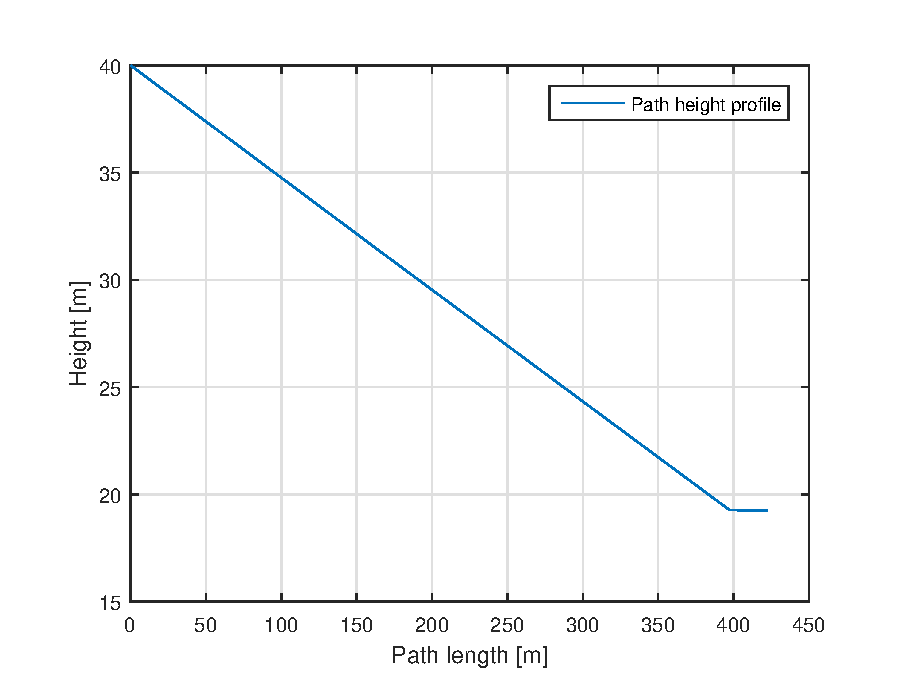
\includegraphics[width=1\textwidth]{figs/SysPlot/heightProfile.eps}
		\caption{Height profile of the landing path}
		\label{Fig:HeightProfile}
\end{figure}
\subsubsection{Spiral path}\label{pp:SpiralPath}
In the case where the approach path has yet to reach the correct heigh at the end of the combined lateral and longitudinal path, a new spiral path is created in order for the approach path to reach the height of the landing path. The spiral path is designed to have the same turning radius, turning direction and decent angle as the approach path. The longitudinal path continues along the spiral until the correct height can be reached with and decent angle equal or less then $\gamma_{d_{Max}}$. Continuing an arc is created such that the path ends with the correct heading. The arc has the same rotation direction as the lateral path, with start point where the correct height was reached and end point of the start of the landing path. The complete approach path combined with the landing path is shown in figure \ref{Fig:LateralPath}.
\begin{figure}[H]
	\centering
		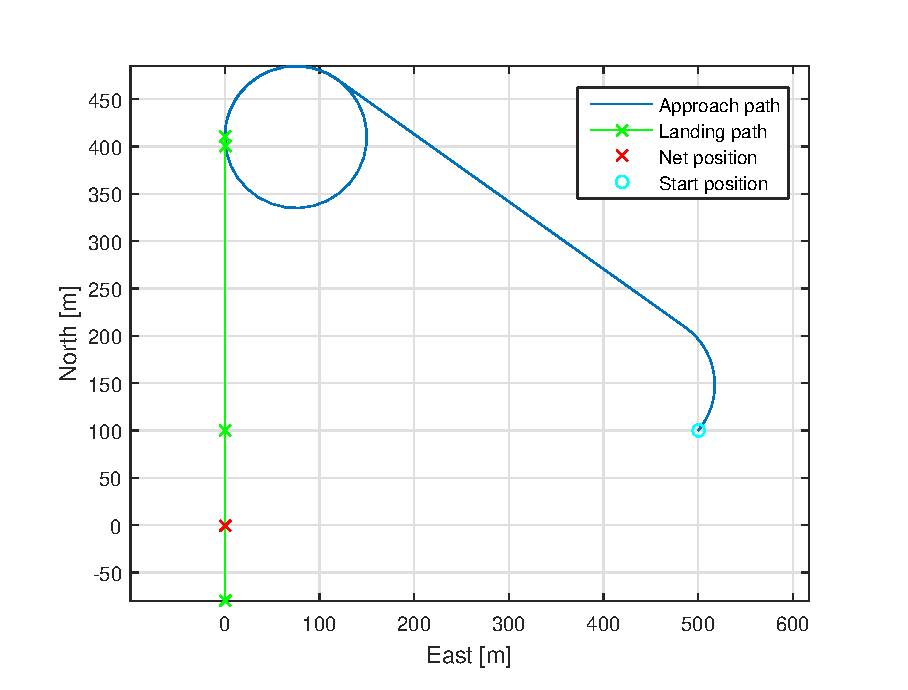
\includegraphics[scale=0.7]{figs/SysPlot/LandingPath.eps}
		\caption{Approach path connected to the landing path}
		\label{Fig:LandingPath}
\end{figure}
\section{Navigation system}
The navigation system consists of two position and velocity measurement system, where one is a high accurate positioning system and the other a reliable backup system. The high accurate positioning system apply \gls{rtk-gnss}, which is able to provide high accurate position solution. The backup positioning system consists of a standard package of standalone \gls{gps} and Inertial Measurement Unit (IMU) together with a Kalman filter, which is a proven reliable system in Ardupilot together with a Pixhawk. Ardupilot and Pixhawk are explained further in section \ref{ss:Pixhawk} and section \ref{ss:ardupilot}. The \gls{rtk-gnss} is subject to drop out, which must be handled by the navigation system. A state switch controller has been created to handle the state switching between \gls{rtk-gps} and the external navigation data. A short drop out of the \gls{rtk-gnss} could be resolved by fusing data from the external navigation source together with previous position solutions from the \gls{rtk-gnss} and create a compensator for the external navigation system. The compensator can then be used to achieve the same accuracy as the \gls{rtk-gnss} for a short period.
\subsection{Position estimation RTK-GPS}\label{ss:rtk-gps}
\acrfull{rtk-gnss} is in \citep{misra2011global} section 7.2.2 defined as a rover that receive raw \gls{gnss} measurements from a reference receiver which is transmitted over a radio link. A key feature with \gls{rtk-gnss} is that the rover is able to estimate the integer ambiguities while moving. The reference receiver is usually defined as a base station and the integer ambiguity is the uncertainty of the number of whole phase cycles between the receiver and a satellite. With the measurements from the base station the rover is able to calculated the distance between itself and the base station, referred to as a baseline. The length of the baseline affects the accuracy of the \gls{rtk-gnss} solution due to increased effect of atmospheric disturbance, which is further described in \ref{Ss:Atmosphere}. With a short baseline, e.g. $1-2 km$ the atmospheric condition can be considered equal for the base station and the rover, which keeps the solution  at centimetre level accuracy. The concept of \gls{rtk-gnss} is depicted in figure \ref{figure:RTK}.
\begin{figure}[H]
	\centering
		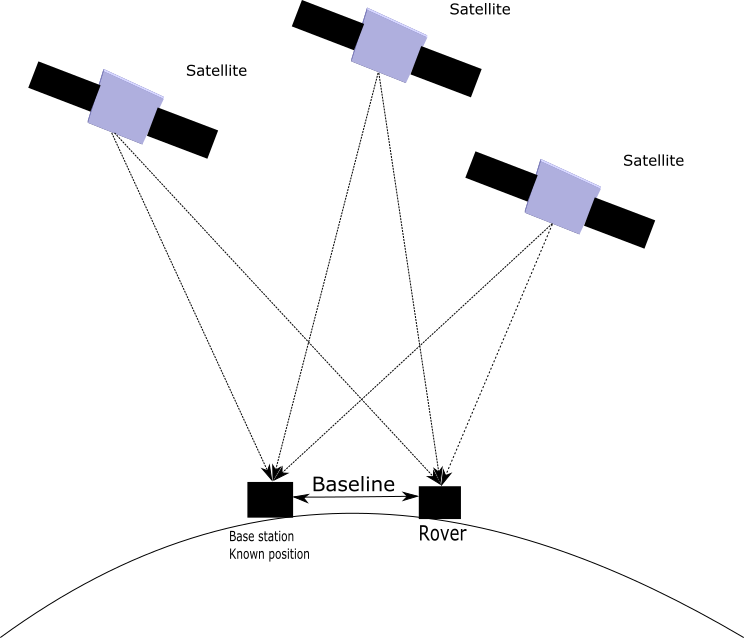
\includegraphics[width=0.7\textwidth]{figs/DGPS.png}
		\caption{Concept figure of \acrfull{rtk-gnss}}
		\label{figure:RTK}
\end{figure}
The ability for the rover to resolve the integer ambiguity is a key feature in \gls{rtk-gnss}. A well used method was presented in the article \citep{teunissen1994new} which decorrelate the integer ambiguities such that an efficient computation of the least square estimate can be performed. The search method is further explained in \citep{teunissen1995least}. An estimate of the integer ambiguity with sufficient high degree of certainty is referred to as a FIX solution, otherwise referred to as a FLOAT solution. When the solution is categorised as FIX the accuracy of the solution is considered on centimetre level, while with a FLOAT solution the accuracy is at a decimetre level. However when a FIX solution is lost, the solution accuracy will not immediately degrade to FLOAT level.

In \gls{rtk-gnss} the position of the base station must be resolved. This can be achieved by either knowing the position beforehand defined as a kinematic configuration. If the base station position is unknown the \gls{rtk-gnss} solver calculates the position on the fly defined as a moving baseline configuration. The unknown position is then calculated as a standalone \gls{gnss} receiver, with the accuracy that entails. Therefore the \gls{rtk-gps} system with a moving baseline configuration can never have better global accuracy then what it will get with a single receiver. The advantage with the moving baseline configuration is that the base station is allowed to move, and with \gls{rtk-gnss} the relative position between the rover and base station can be determined in real time. The advantage with kinematic mode is that it can give a more accurate position estimate, however this require that the base station is known and stationary.
\subsection{Error sources}
In order to get high accuracy in the position estimation the different error sources must be identified and removed if possible. This section will identify some of the most significant error sources that can affect the \gls{gnss} signal and how to remove or mitigate them in the estimation.
\subsubsection{Clock error}
There is drift in both the satellite clock and the receiver clock \citep{misra2011global}. The atomic clock in the satellites makes the clock drift negligible from the user perspective. The receiver clock tend to drift and if not taken into account will cause large deviations in the position estimate from the true position. This error is removed by including a fourth satellite in the position computation. The satellite clock error is given in the satellite message.
\subsubsection{Ionospheric and tropospheric delays}\label{Ss:Atmosphere}
When the \gls{gps} signals travel though the atmosphere there will be a delay caused by the different atmospheric layers \citep{misra2011global}. The atmosphere change the velocity of wave propagation for the radio signal, which results in altered transit time of the signal.
\paragraph{Ionospheric delay}
Gas molecules in the ionosphere become ionized by the ultraviolet rays emitted by the sun and which release free electrons. These electrons can influence electromagnetic wave propagation, such as \gls{gnss} signals. In \citep{vik2014integrated} section 3.5.1 it's stated that the delay caused by the ionosphere usually is in the order of $1-10 $meters. The error can be mitigated by using a double frequency receiver or by applying a mathematical model to estimate the delay. Both those methods are with a single receiver. By including a second receiver in a network, e.g. \gls{rtk-gps}, the \gls{gnss} solution system can assume that both receiver receive signal in the same epoch, which means that the signals have experienced the same delay. The rover is then able to remove the error induced from ionospheric disturbance.
\paragraph{Tropospheric delay}
The tropospheric delay is a function of the local temperature, pressure and relative humidity. The effect of tropospheric delay can  vary from $2.4$ meters to $25$ meters depending on the elevation angle of the satellites,\citep{vik2014integrated} section 3.5.1. The error can be mitigated by applying a mathematical model to estimate the tropospheric delay or by using an elevation mask which neglected all satellites with a elevation angle bellow a certain threshold. Similar to ionospheric delay, tropospheric delay can be removed when using two receivers in a network by assuming that the signal received by both receivers has experienced the same delay. 

\subsubsection{Multipath}
One of the primary source of error in in a \gls{gnss} receiver is multipath \citep{misra2011global}. Multipath happens when the satellite signal is reflected by a nearby surface before if reaches the \gls{gnss} antenna. The delay introduced in the signal can make the receiver believe that its position is several meters away form its true position. The easiest way to mitigated multipath is to place the antenna at an open location with no tall structures nearby. The effect can also be mitigated by choosing an antenna with good multipath rejection capability. Multipath error is uncorrelated between receivers, thus the local receiver must be able to correct for multipath error locally.

\subsection{Navigation state control system}\label{S:NavState}
The navigation state control system manage the current state of the navigation system, which controls the \gls{rtk-gnss} usage and is responsible for dispatching the current state of the \gls{uav} to the rest of the DUNE system. A state diagram of the navigation state control system is shown in figure \ref{Fig:NavState}, which show the state interaction, trigger events and state entry actions. The entry actions ensure that only functionality that is connected to the current state is active      and that monitors are updated with the state switch. The navigation state control system is designed to function without \gls{rtk-gnss} available, which makes the navigation system independent from the \gls{rtk-gnss} system. This is a requirement for the navigation system since it should function in a \gls{uav} where \gls{rtk-gnss} is not present.

In order for the navigation system to switch state into "Rtk ready" the \gls{rtk-gps} message must be considered valid. This is described in section \ref{ss:RTK-GPS system}. In addition the \gls{rtk-gps} solution type must be FIX for $x$ seconds such that the \gls{rtk-gnss} solution can be considered highly accurate. For the navigation state control system to switch to \gls{rtk-gnss} the user has to specify \gls{rtk-gnss} usage from the command and control software used to monitor the \gls{uav}. In the case where a loss of \gls{rtk-gnss} is experienced the short \gls{rtk-gnss} compensator will be activated to prevent the loss of \gls{rtk-gnss} accuracy, thus prolonging the availability of the \gls{rtk-gnss}. This state will be further described in section \ref{ss:ShortLoss}. A summary of the states in the navigation state control system is given in table \ref{Tb:StateDescription}.
\begin{figure}[H]
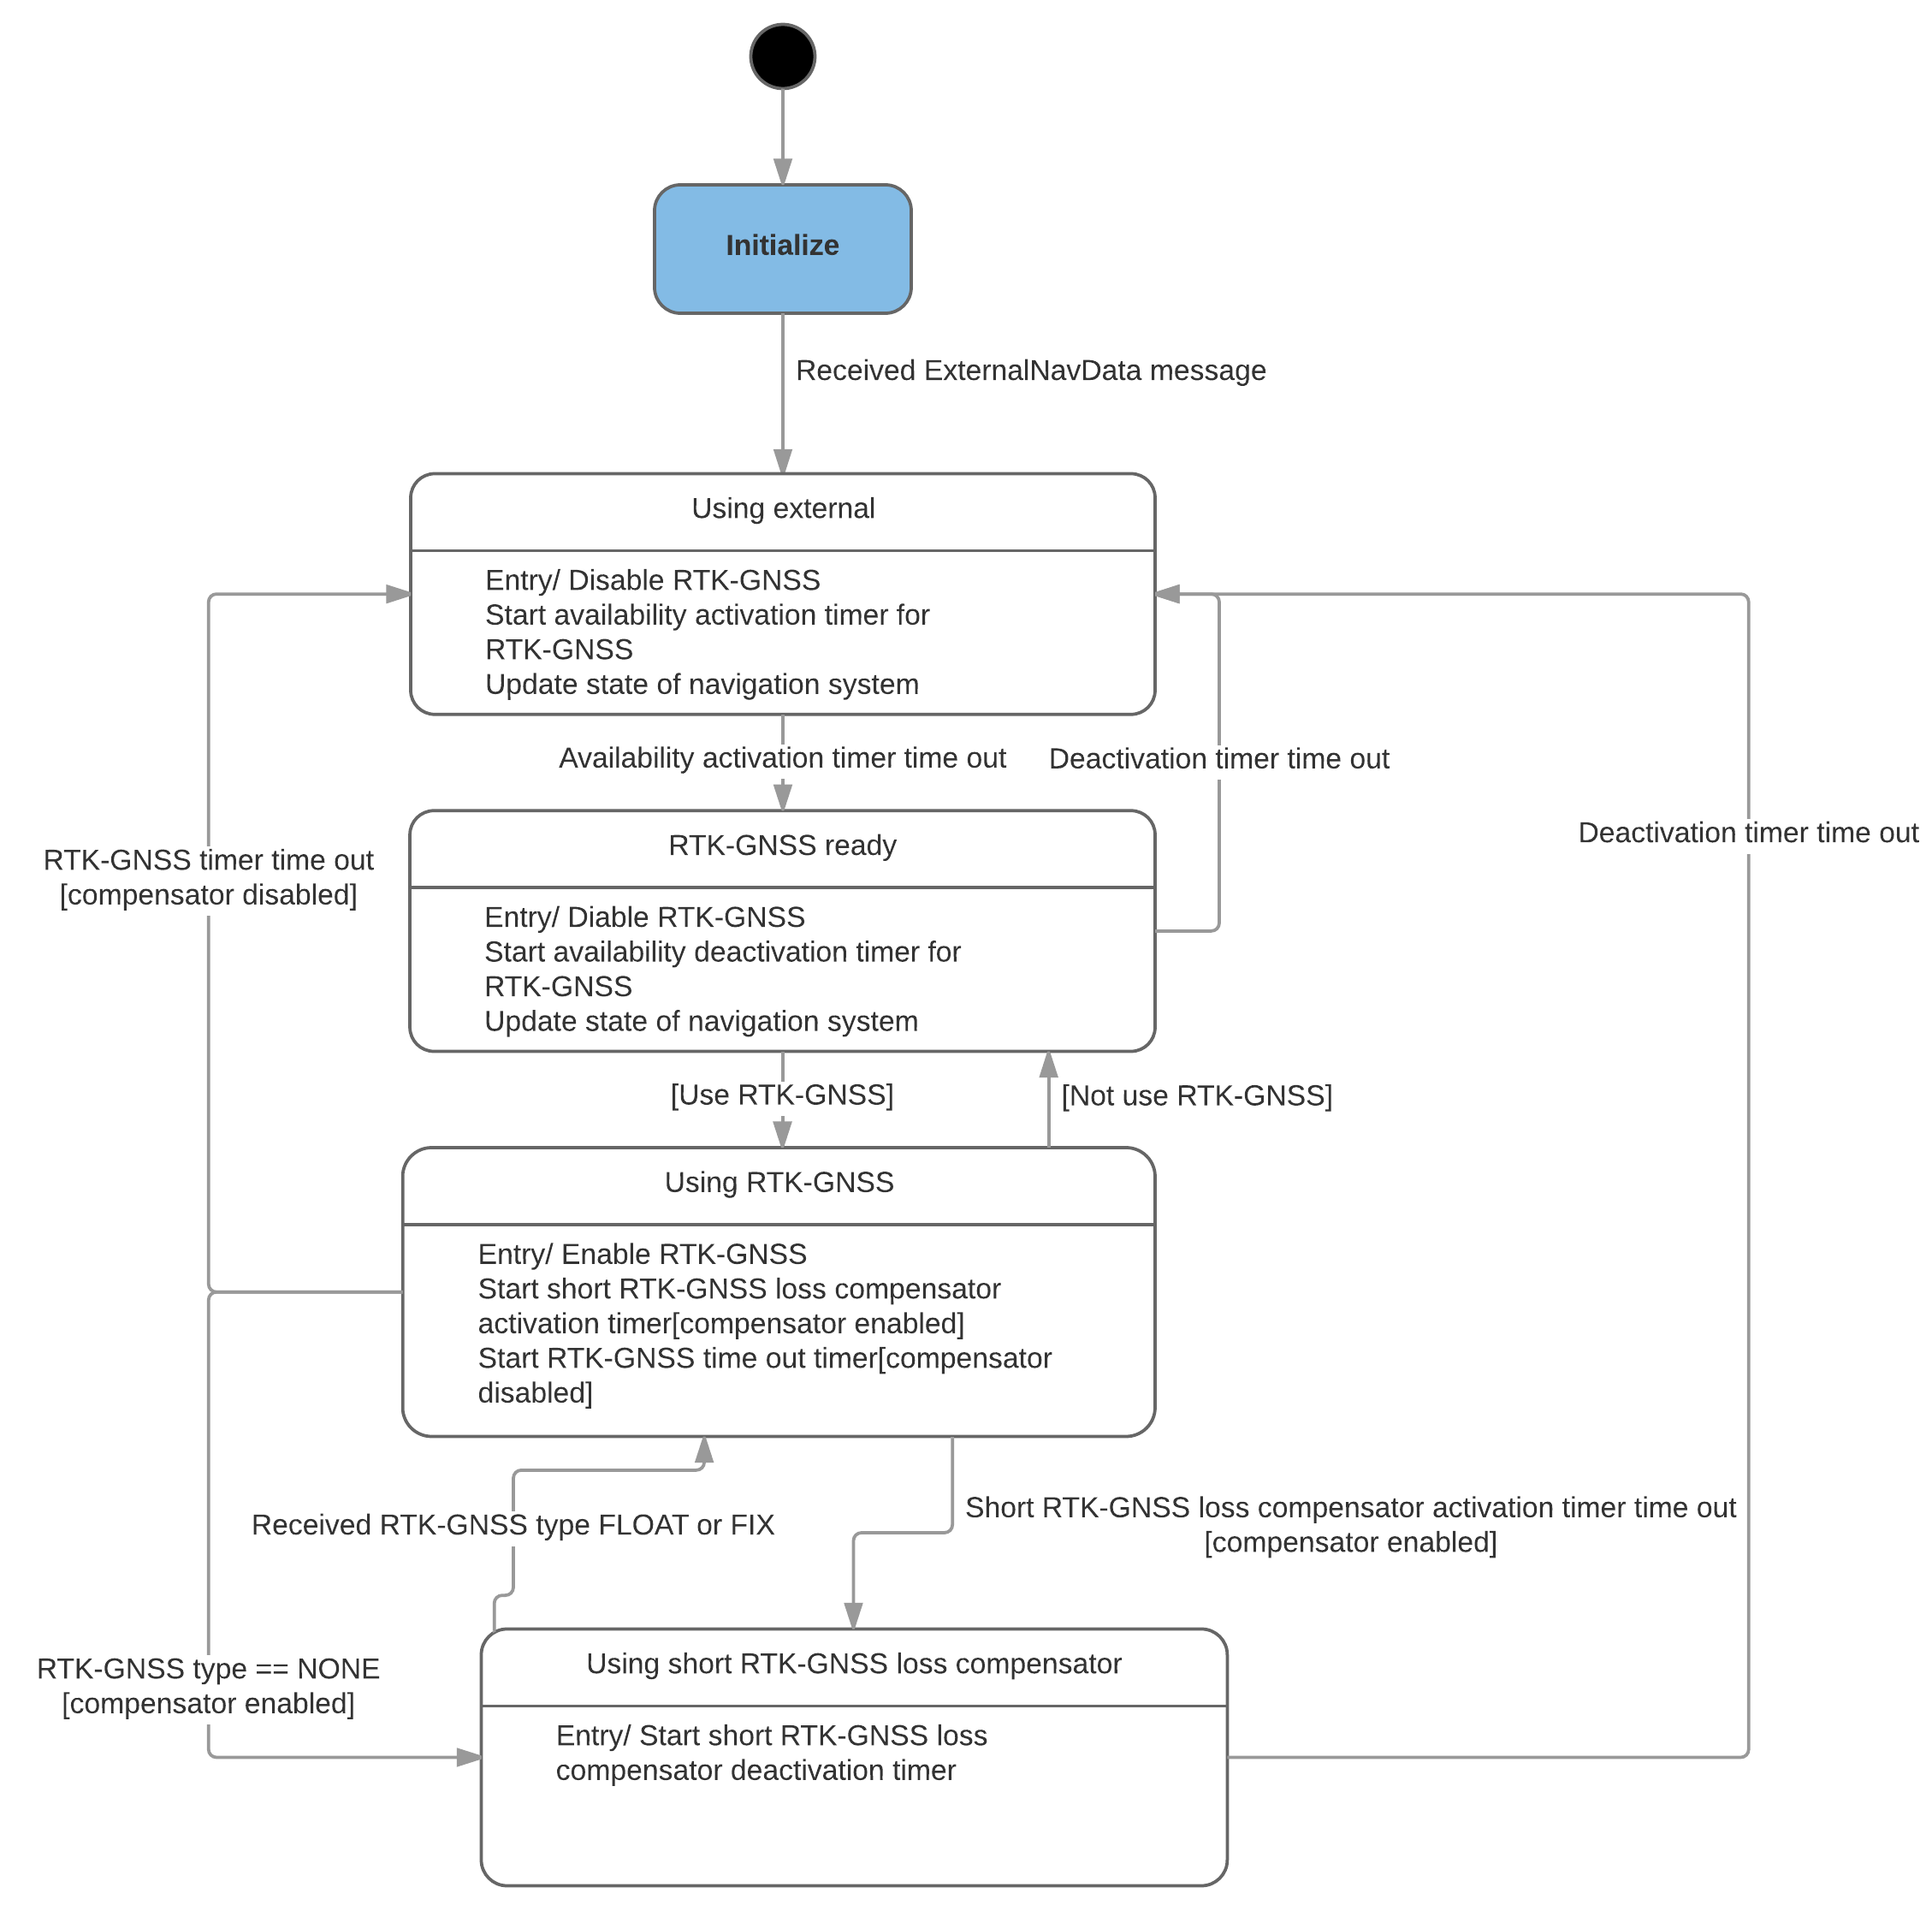
\includegraphics[scale=0.18]{figs/NavigationStateControl.png}
\caption{State machine in the DUNE Navigation task}
\label{Fig:NavState}
\end{figure}
\begin{table}[H]
\begin{tabular}{ | p{3cm} | p{8cm} |}
	\hline 
	\textbf{State}						& \textbf{Description} \\ \hline
	Initialize							& The task starting up\\ \hline
	Using external						& The navigation task apply the external navigation source in the state message\\ \hline
	\gls{rtk-gnss} ready							& The \gls{rtk-gnss} is ready for use, however the external navigation source is still used\\ \hline
	Using \gls{rtk-gnss}							& The navigation task apply the \gls{rtk-gnss} in the state message\\ \hline
	Using short \gls{rtk-gnss} loss compensator	& The navigation task apply the external navigation source with a compensation term to reduce the effect of \gls{rtk-gnss} loss. \\ \hline
\end{tabular}
\caption{States in the navigation system with description}
\label{Tb:StateDescription}
\end{table}
\subsubsection{Short loss of \gls{rtk-gnss}}\label{ss:ShortLoss}
The short \gls{rtk-gnss} loss compensator is design to prevent loss of position accuracy in the \gls{uav} navigation system during \gls{rtk-gnss} drop out. The compensator is based on that the position solution from the external navigation system is almost constant with respect to the \gls{rtk-gnss} solution. As seen in figure \ref{Fig:RTKExternal} the position of the \gls{rtk-gnss} and the external navigation system remain close to each other, given that the \gls{rtk-gnss} has a FIX solution. 
\begin{figure}[H]
\centering
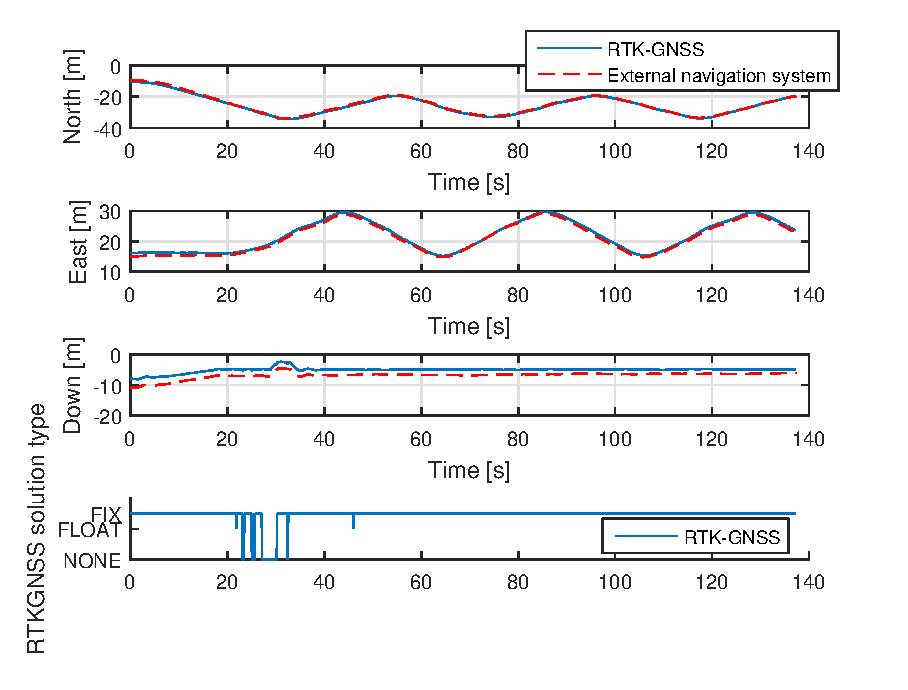
\includegraphics[scale=0.8]{figs/Experiment/RtkExternal.eps}
\caption{Plot where the \gls{rtk-gnss} solution is displayed together with the position solution from the external navigation system, include the solution type of the \gls{rtk-gnss} system.}
\label{Fig:RTKExternal}
\end{figure}
The slow moving difference between the \gls{rtk-gnss} and external navigation system position solution is confirmed in figure \ref{Fig:RtkExtDiff}.
\begin{figure}[H]
\centering
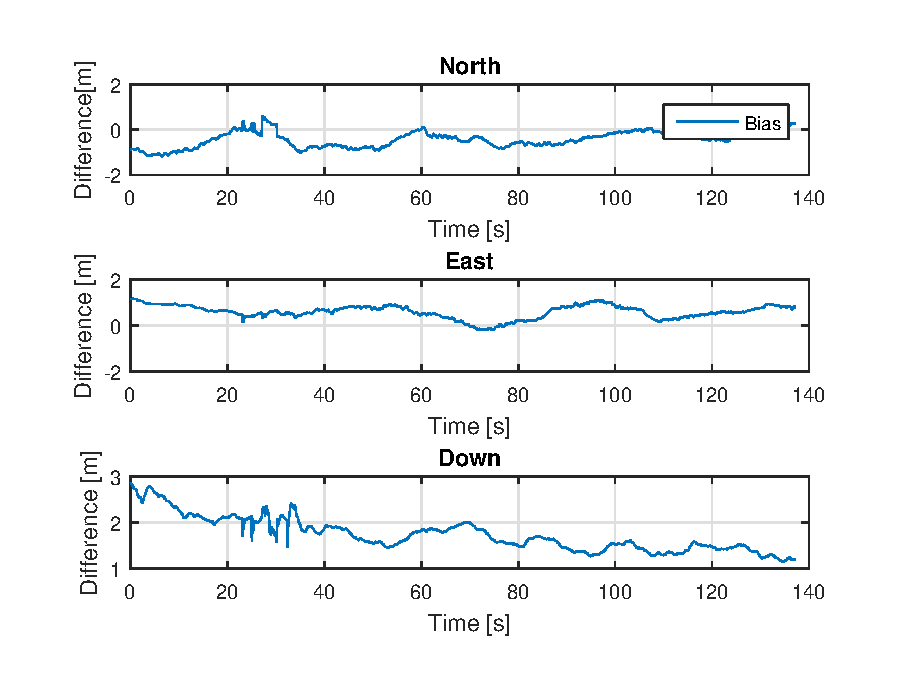
\includegraphics[scale=0.8]{figs/Experiment/biasShow.eps}
\caption{The difference between the \gls{rtk-gnss} solution and the external navigation system position solution}
\label{Fig:RtkExtDiff}
\end{figure}
Therefore the average difference between the \gls{rtk-gnss} position solution and the external navigation system should be able to move the external navigation position solution closer to the \gls{rtk-gps} position solution. The short loss compensator is given as:
\begin{align}
\mathbf{e}(n) &= \mathbf{p}_1(n) - \mathbf{p}_2(n)\\
\mathbf{\delta} &= \frac{1}{N}\sum_{n=0}^N(\mathbf{e}(n))
\end{align}
where $\mathbf{p}_1(n)$ and $\mathbf{p}_2(n)$ is the position solution sample for the \gls{rtk-gnss} system and the external navigation system respectfully. $N$ is the total number of samples with $n\in [0,N-1]$ as the counting variable. Adding $\mathbf{\delta}$ to the external navigation position with the assumption of slow varying bias between the two position solution gives:
\begin{equation}
\mathbf{p}_2(t) + \mathbf{\delta} \rightarrow \mathbf{p}_1(t)
\end{equation}
where $\mathbf{p}_1(t)$ and $\mathbf{p}_2(t)$ is the current position solution for the \gls{rtk-gnss} system and the external navigation system respectively. The short loss \gls{rtk-gnss} compensator will be triggered if there is a delay in the \gls{rtk-gnss} system or an temporary drop out occurs. The output frequency of the short loss compensator is set to be the same as the \gls{rtk-gnss} system and is estimated by comparing the time each \gls{rtk-gnss} message is dispatched. This results in prolonging the time where the \gls{rtk-gnss} is available for the navigation system and ensure a stable output frequency from the \gls{uav} navigation system. The compensator is designed to prevent mission abortion and make the \gls{rtk-gnss} system more robust.
\section{Summary}
This chapter has presented a system description of both a landing plan generator and a navigation system with robust \gls{rtk-gnss}. The landing plan presented is separated into two parts; the landing path and the approach path. The landing path is a straight line path towards the net, and the approach path is a combination of Dubins path in the lateral plane and straight line path in the longitudinal plane. The approach path is designed to guaranty that \gls{uav} has a flyable path which enables the \gls{uav} to enter the landing path at the correct height with the correct orientation from any initial position.

The \gls{uav} navigation system has been designed with a navigation state control system used to control the current state of the source of the navigation data. Currently the different navigation source available to the \gls{uav} is an external navigation system and a \gls{rtk-gnss} system. In order to prolong the availability of the \gls{rtk-gnss} during short drop outs a short \gls{rtk-gnss} loss compensator system is presented used to compensate the external navigation system position solution in order for the \gls{uav} navigation system to keep the a \gls{rtk-gnss} accuracy level during a \gls{rtk-gnss} drop out.